\documentclass{standalone}
\usepackage{tikz}
\usetikzlibrary{patterns, positioning}
\usepackage[sfdefault]{ClearSans} %% option 'sfdefault' activates Clear Sans as the default text font
\usepackage[T1]{fontenc}

\begin{document}
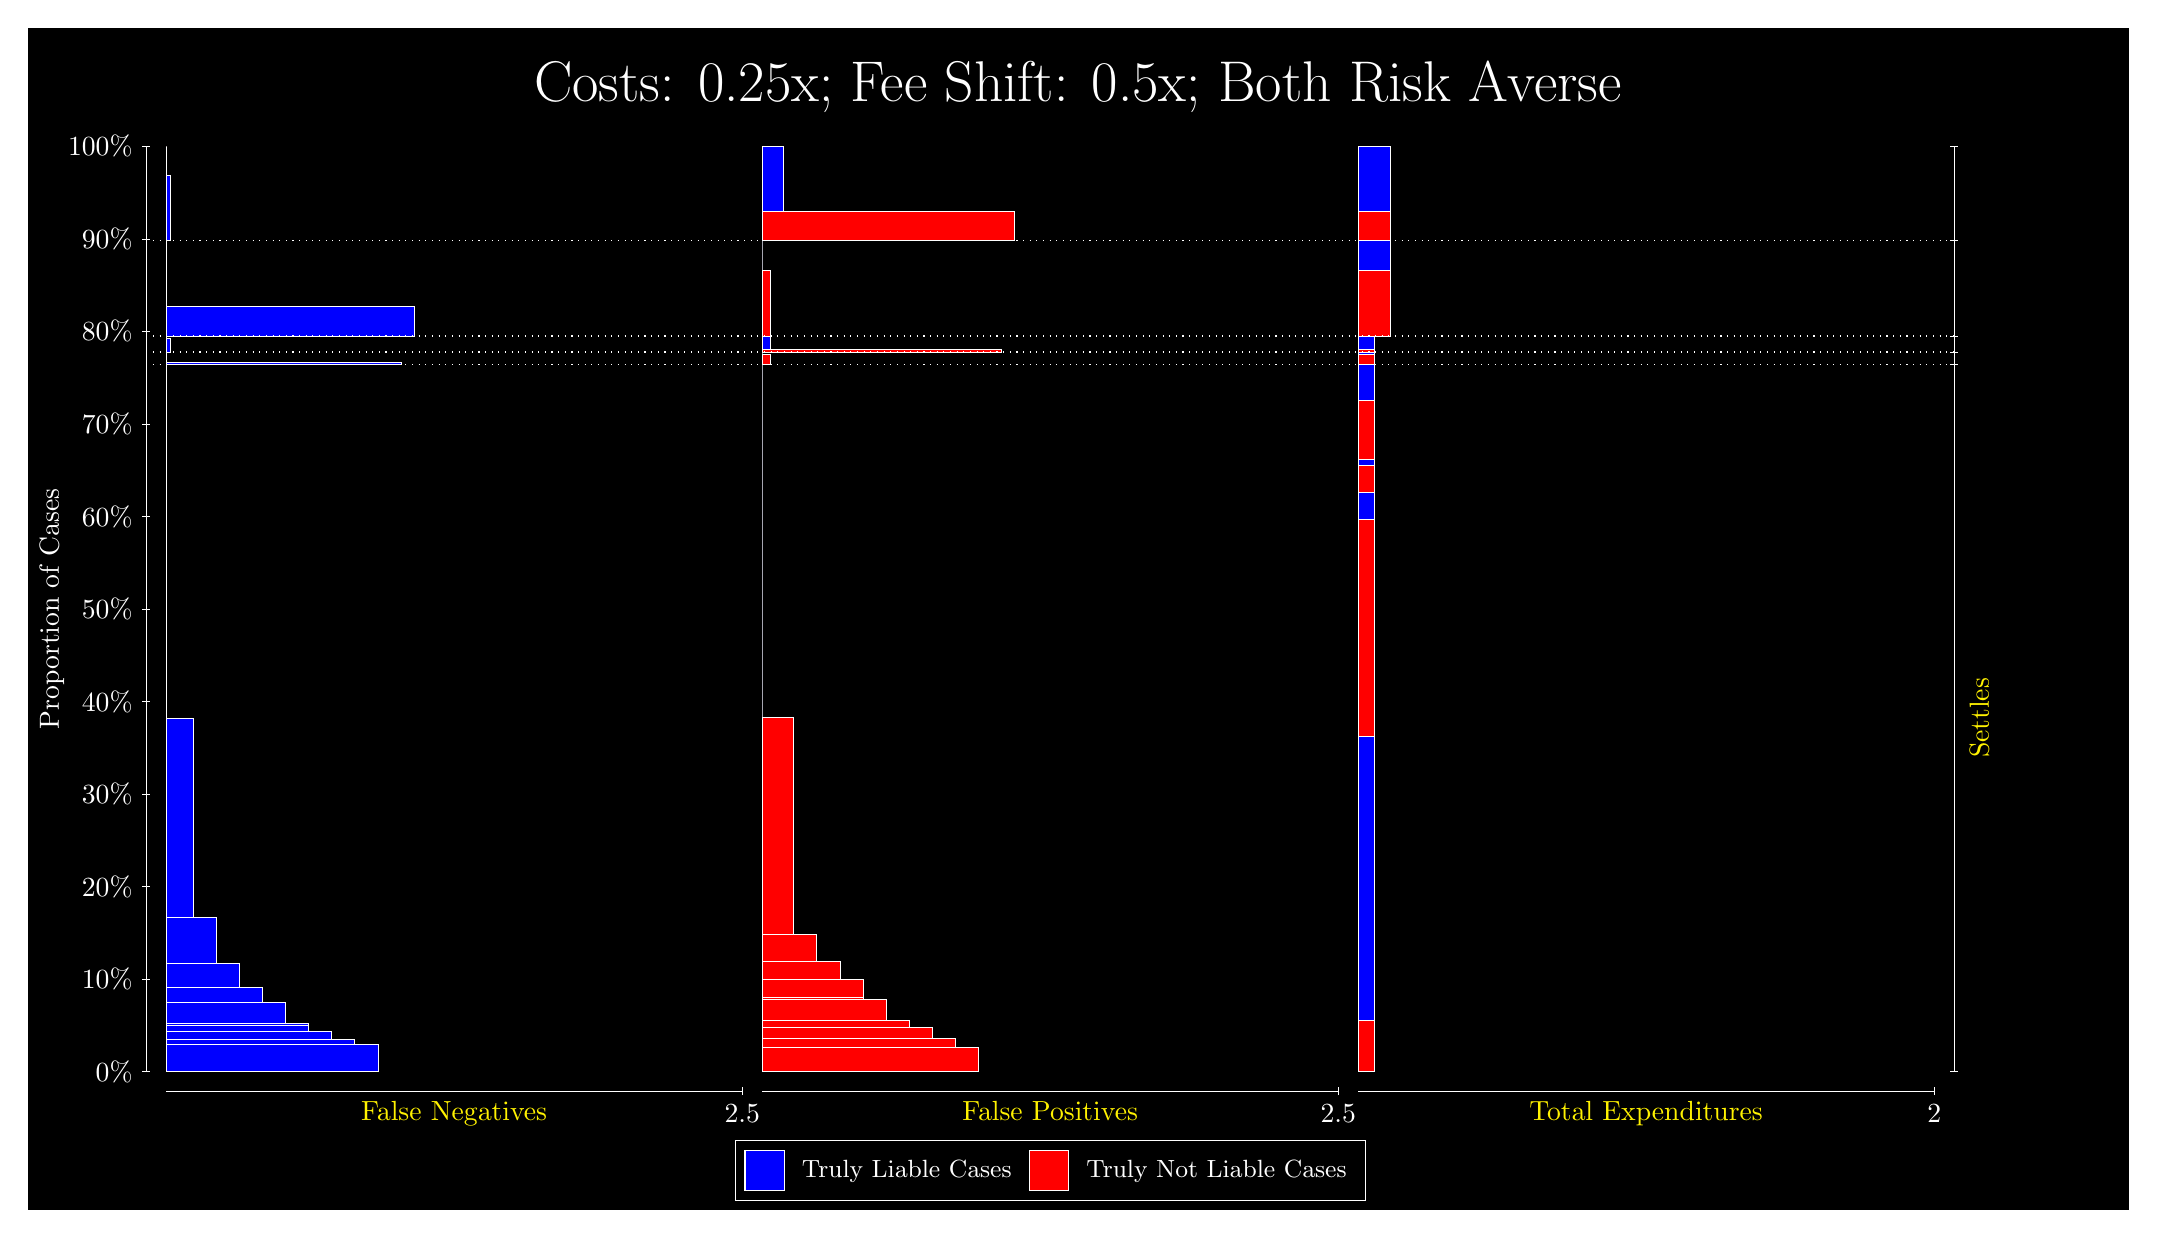
\begin{tikzpicture}
\draw[fill=black] (0,0) rectangle (26.667,15);
\draw[text=white] (0,13.5) rectangle (26.667,15) node[midway] {\huge Costs: 0.25x; Fee Shift: 0.5x; Both Risk Averse};
\draw[white, very thin] (1.5,1.75) -- (1.5,13.5);
\node[rotate=90, text=white, anchor=center] at (0.3, 7.625) {Proportion of Cases};
\draw[white, very thin] (1.45,1.75) -- (1.55,1.75);
\node[text=white, anchor=east] at (1.45, 1.75) {0\%};
\draw[white, very thin] (1.45,2.925) -- (1.55,2.925);
\node[text=white, anchor=east] at (1.45, 2.925) {10\%};
\draw[white, very thin] (1.45,4.1) -- (1.55,4.1);
\node[text=white, anchor=east] at (1.45, 4.1) {20\%};
\draw[white, very thin] (1.45,5.275) -- (1.55,5.275);
\node[text=white, anchor=east] at (1.45, 5.275) {30\%};
\draw[white, very thin] (1.45,6.45) -- (1.55,6.45);
\node[text=white, anchor=east] at (1.45, 6.45) {40\%};
\draw[white, very thin] (1.45,7.625) -- (1.55,7.625);
\node[text=white, anchor=east] at (1.45, 7.625) {50\%};
\draw[white, very thin] (1.45,8.8) -- (1.55,8.8);
\node[text=white, anchor=east] at (1.45, 8.8) {60\%};
\draw[white, very thin] (1.45,9.975) -- (1.55,9.975);
\node[text=white, anchor=east] at (1.45, 9.975) {70\%};
\draw[white, very thin] (1.45,11.15) -- (1.55,11.15);
\node[text=white, anchor=east] at (1.45, 11.15) {80\%};
\draw[white, very thin] (1.45,12.325) -- (1.55,12.325);
\node[text=white, anchor=east] at (1.45, 12.325) {90\%};
\draw[white, very thin] (1.45,13.5) -- (1.55,13.5);
\node[text=white, anchor=east] at (1.45, 13.5) {100\%};

\draw[white, very thin] (24.457,1.75) -- (24.457,13.5);
\draw[white, very thin] (24.407,1.75) -- (24.507,1.75);
\node[anchor=west] at (24.407, 1.75) {};
\draw[white, very thin] (24.407,10.734) -- (24.507,10.734);
\node[anchor=west] at (24.407, 10.734) {};
\draw[white, very thin] (24.407,10.888) -- (24.507,10.888);
\node[anchor=west] at (24.407, 10.888) {};
\draw[white, very thin] (24.407,11.091) -- (24.507,11.091);
\node[anchor=west] at (24.407, 11.091) {};
\draw[white, very thin] (24.407,12.303) -- (24.507,12.303);
\node[anchor=west] at (24.407, 12.303) {};
\draw[white, very thin] (24.407,13.5) -- (24.507,13.5);
\node[anchor=west] at (24.407, 13.5) {};

\draw[white, very thin, fill=blue] (1.75,1.75) rectangle (4.4397,2.0932);
\draw[white, very thin, fill=blue] (1.75,2.0932) rectangle (4.1469,2.1649);
\draw[white, very thin, fill=blue] (1.75,2.1649) rectangle (3.8542,2.2577);
\draw[white, very thin, fill=blue] (1.75,2.2577) rectangle (3.5614,2.3399);
\draw[white, very thin, fill=blue] (1.75,2.3399) rectangle (3.5614,2.3677);
\draw[white, very thin, fill=blue] (1.75,2.3677) rectangle (3.2687,2.6284);
\draw[white, very thin, fill=blue] (1.75,2.6284) rectangle (2.9759,2.8228);
\draw[white, very thin, fill=blue] (1.75,2.8228) rectangle (2.6832,3.1242);
\draw[white, very thin, fill=blue] (1.75,3.1242) rectangle (2.3904,3.7109);
\draw[white, very thin, fill=blue] (1.75,3.7109) rectangle (2.0976,6.2329);
\draw[white, very thin, fill=red] (1.75,6.2329) rectangle (1.75,10.734);
\draw[white, very thin, fill=blue] (1.75,10.734) rectangle (4.7324,10.759);
\draw[white, very thin, fill=red] (1.75,10.759) rectangle (1.75,10.888);
\draw[white, very thin, fill=blue] (1.75,10.888) rectangle (1.8049,11.058);
\draw[white, very thin, fill=red] (1.75,11.058) rectangle (1.75,11.091);
\draw[white, very thin, fill=blue] (1.75,11.091) rectangle (4.8971,11.464);
\draw[white, very thin, fill=red] (1.75,11.464) rectangle (1.75,12.303);
\draw[white, very thin, fill=blue] (1.75,12.303) rectangle (1.8049,13.128);
\draw[white, very thin, fill=red] (1.75,13.128) rectangle (1.75,13.5);
\draw[white, very thin, fill=red] (9.3189,1.75) rectangle (12.063,2.0518);
\draw[white, very thin, fill=red] (9.3189,2.0518) rectangle (11.771,2.175);
\draw[white, very thin, fill=red] (9.3189,2.175) rectangle (11.478,2.3057);
\draw[white, very thin, fill=red] (9.3189,2.3057) rectangle (11.185,2.4036);
\draw[white, very thin, fill=red] (9.3189,2.4036) rectangle (10.892,2.663);
\draw[white, very thin, fill=red] (9.3189,2.663) rectangle (10.6,2.6918);
\draw[white, very thin, fill=red] (9.3189,2.6918) rectangle (10.6,2.9193);
\draw[white, very thin, fill=red] (9.3189,2.9193) rectangle (10.307,3.154);
\draw[white, very thin, fill=red] (9.3189,3.154) rectangle (10.014,3.4973);
\draw[white, very thin, fill=red] (9.3189,3.4973) rectangle (9.7214,6.251);
\draw[white, very thin, fill=blue] (9.3189,6.251) rectangle (9.3189,10.734);
\draw[white, very thin, fill=red] (9.3189,10.734) rectangle (9.4287,10.863);
\draw[white, very thin, fill=blue] (9.3189,10.863) rectangle (9.3189,10.888);
\draw[white, very thin, fill=red] (9.3189,10.888) rectangle (12.356,10.921);
\draw[white, very thin, fill=blue] (9.3189,10.921) rectangle (9.4287,11.091);
\draw[white, very thin, fill=red] (9.3189,11.091) rectangle (9.4287,11.93);
\draw[white, very thin, fill=blue] (9.3189,11.93) rectangle (9.3189,12.303);
\draw[white, very thin, fill=red] (9.3189,12.303) rectangle (12.521,12.675);
\draw[white, very thin, fill=blue] (9.3189,12.675) rectangle (9.5933,13.5);
\draw[white, very thin, fill=red] (16.888,1.75) rectangle (17.094,2.4036);
\draw[white, very thin, fill=blue] (16.888,2.4036) rectangle (17.094,6.0081);
\draw[white, very thin, fill=red] (16.888,6.0081) rectangle (17.094,8.7618);
\draw[white, very thin, fill=blue] (16.888,8.7618) rectangle (17.094,9.105);
\draw[white, very thin, fill=red] (16.888,9.105) rectangle (17.094,9.4483);
\draw[white, very thin, fill=blue] (16.888,9.4483) rectangle (17.094,9.52);
\draw[white, very thin, fill=red] (16.888,9.52) rectangle (17.094,10.27);
\draw[white, very thin, fill=blue] (16.888,10.27) rectangle (17.094,10.734);
\draw[white, very thin, fill=red] (16.888,10.734) rectangle (17.094,10.863);
\draw[white, very thin, fill=blue] (16.888,10.863) rectangle (17.094,10.888);
\draw[white, very thin, fill=red] (16.888,10.888) rectangle (17.094,10.921);
\draw[white, very thin, fill=blue] (16.888,10.921) rectangle (17.094,11.091);
\draw[white, very thin, fill=red] (16.888,11.091) rectangle (17.299,11.93);
\draw[white, very thin, fill=blue] (16.888,11.93) rectangle (17.299,12.303);
\draw[white, very thin, fill=red] (16.888,12.303) rectangle (17.299,12.675);
\draw[white, very thin, fill=blue] (16.888,12.675) rectangle (17.299,13.5);
\draw[white, dotted] (1.5,10.734) -- (24.457,10.734);
\draw[white, dotted] (1.5,10.888) -- (24.457,10.888);
\draw[white, dotted] (1.5,11.091) -- (24.457,11.091);
\draw[white, dotted] (1.5,12.303) -- (24.457,12.303);
\draw[white, very thin] (1.75,1.5) -- (9.0689,1.5);
\node[text=yellow, anchor=north] at (5.4094, 1.5) {False Negatives};
\draw[white, very thin] (9.0689,1.45) -- (9.0689,1.55);
\node[text=white, anchor=north] at (9.0689, 1.45) {2.5};

\draw[white, very thin] (9.3189,1.5) -- (16.638,1.5);
\node[text=yellow, anchor=north] at (12.978, 1.5) {False Positives};
\draw[white, very thin] (16.638,1.45) -- (16.638,1.55);
\node[text=white, anchor=north] at (16.638, 1.45) {2.5};

\draw[white, very thin] (16.888,1.5) -- (24.207,1.5);
\node[text=yellow, anchor=north] at (20.547, 1.5) {Total Expenditures};
\draw[white, very thin] (24.207,1.45) -- (24.207,1.55);
\node[text=white, anchor=north] at (24.207, 1.45) {2};

\node[text=yellow, centered, rotate=90] at (24.777, 6.2419) {Settles};





\draw (12.978300999999998,1.5) node[draw=none] (baseCoordinate) {};
\begin{scope}[align=center]
        \matrix[scale=0.5, draw=white, below=0.5cm of baseCoordinate, nodes={draw}, column sep=0.1cm]{
            \node[rectangle, draw, minimum width=0.5cm, minimum height=0.5cm, fill=blue] {}; &
            \node[draw=none, font=\small, text=white] (B) {Truly Liable Cases}; &
            \node[rectangle, draw, minimum width=0.5cm, minimum height=0.5cm, fill=red] {}; &
            \node[draw=none, font=\small, text=white] (B) {Truly Not Liable Cases}; \\
            };
\end{scope}

\end{tikzpicture}
\end{document}